\documentclass[10pt,journal,compsoc]{IEEEtran}


\ifCLASSOPTIONcompsoc

\fi

\usepackage{graphicx}

\newcommand\MYhyperrefoptions{bookmarks=true,bookmarksnumbered=true,
pdfpagemode={UseOutlines},plainpages=false,pdfpagelabels=true,
colorlinks=true,linkcolor={black},citecolor={black},urlcolor={black},
pdftitle={Bare Demo of IEEEtran.cls for Computer Society Journals},%<!CHANGE!
pdfsubject={Typesetting},%<!CHANGE!
pdfauthor={Michael D. Shell},%<!CHANGE!
pdfkeywords={Computer Society, IEEEtran, journal, LaTeX, paper,
             template}}%<^!CHANGE!

\hyphenation{op-tical net-works semi-conduc-tor}


\begin{document}

\title{Mobile Service Composition over Oppotunistic Networks: An Energy Consumption Perspective}

\author{Qinglan~Peng,~\IEEEmembership{Member,~IEEE,}
        John~Doe,~\IEEEmembership{Fellow,~OSA,}
        and~Jane~Doe,~\IEEEmembership{Life~Fellow,~IEEE}% <-this % stops a space
\IEEEcompsocitemizethanks{\IEEEcompsocthanksitem M. Shell was with the Department
of Electrical and Computer Engineering, Georgia Institute of Technology, Atlanta,
GA, 30332.\protect\\
% note need leading \protect in front of \\ to get a newline within \thanks as
% \\ is fragile and will error, could use \hfil\break instead.
E-mail: see http://www.michaelshell.org/contact.html
\IEEEcompsocthanksitem J. Doe and J. Doe are with Anonymous University.}% <-this % stops a space
\thanks{Manuscript received April 19, 2005; revised August 26, 2015.}}



% The paper headers
\markboth{Journal of \LaTeX\ Class Files,~Vol.~14, No.~8, August~2015}%
{Shell \MakeLowercase{\textit{et al.}}: Bare Advanced Demo of IEEEtran.cls for IEEE Computer Society Journals}

\IEEEtitleabstractindextext{%
\begin{abstract}
The abstract goes here.
\end{abstract}

% Note that keywords are not normally used for peerreview papers.
\begin{IEEEkeywords}
Computer Society, IEEE, IEEEtran, journal, \LaTeX, paper, template.
\end{IEEEkeywords}}


% make the title area
\maketitle



\IEEEdisplaynontitleabstractindextext

\IEEEpeerreviewmaketitle


\ifCLASSOPTIONcompsoc
\IEEEraisesectionheading{\section{Introduction}\label{sec:introduction}}
\else
\section{Introduction}
\label{sec:introduction}
\fi


\IEEEPARstart{I}{n recent} years, service-oriented computing has become an increasingly important computing paradigm to develop
and integrate distributed enterprise information systems [T]. With the rapid developments in mobile devices and wireless technologies, Web services are no longer limited to traditional platforms and they are becoming more flexible and com- plex. The manufacturers of mobile devices have also recently achieved breakthroughs to extend mobile devices’ capabilities in terms of memory, computational power, storage capacity, and display screens as well as expand their capabilities and functionalities with other integrated devices, such as built-in cameras, infrared ports, and Bluetooth technology [T]. As aresult, theglobal interestof mobileapplications isonthe rise. Both researchers and industrial companies are inspired to pave the road for mobile Web service provisioning [T][2].

Opportunistic computing provides an appealing alternative to the mobile computing cloud by allowing devices to join forces and leverage heterogeneous resources from other devices[1 abstract].

To complement online mobile crowdsourcing services, in this paper we advocate Crowd Foraging,a QoS-oriented selforganized mobile crowdsourcing framework, where a mobile user can self-organize her task crowdsourcing in a proactive manner by leveraging a massive crowd of opportunistically encountered mobile human workers in realtime. Its main rationality is four-fold. First, opportunistic user encounters are prevalent and sufficient in daily life [T], which offers plenty of opportunities to exploit nearby human intelli- gence for task solving [T], [T], [T]. Second, many mobile crowdsourcing tasks require local knowledge and information (e.g., location-based content sensing [T], [T], [T] and content transmission [T]–[T]), and hence nearby human workers are more adept at executing them than the online workers. Third, D2D communications such as Bluetooth, WiFi-direct and LTE-D2D are promising to replenish traditional cellular communications in terms of user throughput increase, cellular traffic reduction and network coverage extension [T]. At last, this framework shares the similar spirit with the emerging paradigm “cyber foraging” over opportunistic networks, such that mobile users opportunistically exploit nearby device resources to facilitate their computational task processing [T][3].

Because the pervasive vision revolves around the human user, it can only be achieved by a flexible networking paradigm that adapts to the user instead of expecting the user to adapt. Human users move around freely and cannot be expected to always be within range of an access point or a mesh router. On the other hand, humans are social by nature, and they can very well be expected to come in contact with each other with a relatively high frequency; it is this very expectation that constitutes the basic tenet of opportunistic networking [1].


% \hfill mds
 
% \hfill August 26, 2015

\subsection{Mobile Web Service}
Mobile Web services are deployed on mobile devices and
provisioned over wireless networks, and devices may play the roles of consumers, brokers, or providers. Their role as aWeb service requester isfundamental. Shifting such a role from a requester to a provider, however, is feasible only if mobile devices can offer standard Web services with accept- able performance while making negligible impact on their regular usage. The concept of mobile Web services was first introduced as a computing paradigm in the early twenty-first century [T]. It brought many challenges to traditional ser- vice computing techniques mainly due to their technological limitations, summarized as follows.


\emph{1) Mobility:} Mobile devices frequently change network operators and may handover between different technologies within the same network. Also, because they are expected to experience frequent link failures, services they provide may become temporarily unreachable. This presents major chal- lenges for providing reliable Web services in highly dynamic mobile wireless environments. 

\emph{2) Limited Resources:} Although the capabilities of mobile devices have improved in terms of processing power, mem- ory space, and embedded sensors, they continue to lag behind other forms of computing devices. Mobile devices (smartphones in particular) are still recognized as resource- constrained computing devices [T]. Battery power is the number one limited resource in mobile phones, which remains a major challenge for potential growth of mobile computing [T]. Recent developments in mobile computing and growing popularity of mobile applications outpace what current battery technologies can provide.

\emph{3) Addressability:} 

\emph{4) Scalability:} 

Due to the above characteristics, the existing service com-
puting protocols and mechanisms can be hardly utilized for mobile Web services. Therefore, it is essential to study new protocols and mechanisms that are more suitable for mobile domains. In this paper, we mainly target at the service selection by considering user mobility [2].


\subsection{Motivation Scenario}

\subsection{Contributions}
To address the aforementioned challenges and concerns,
we propose a new approach for service selections and com- positions in mobile environments. The main contributions are:

1) We propose an architecture for mobile service provision [mobile service sharing community (MSSC)] to address the problem of service selection for mobile service com- position in the mobile community where both service requesters and providers are nonstationary. In such com- munity, mobile users can share mobile services through their mobile devices in specific areas.

2) For MSSC, we propose a mobility model to describe mobile user moving behavior. The model is extended from the random waypoint (RWP) model.

3) Based on MSSC and the proposed mobility model, we transfer the mobility-aware service composition prob- lem to an optimization problem and propose to utilize the Krill-Herd (KH) algorithm to solve it. We conduct aseries of evaluations to validate that our algorithmis approximately optimal and performs much better than other standard composition approaches. We compare it with other population-based optimization methods for both optimality and scalability.

The remainder of this paper is organized as follows.
Section II reviews the related work. Section III introduces the MSSC architecture. Section IV describes our approach to make service compositions. Section V presents experimental results. Section VI concludes this paper.





\section{RELATED WORK AND COMPARISON}
Service composition is a significant area of research. As our proposal targets the problem of mobile service composition, we first briefly review the work on how to make such com- position in traditional Internet environment, then we review some recent work on it in dynamic/mobile environments.
\subsection{Traditional Web Service Composition}
\subsection{Mobile Web Service Composition}


\section{MOBILE OPPORTUNISTIC NETWORK}

\begin{figure}[!t]
\centering
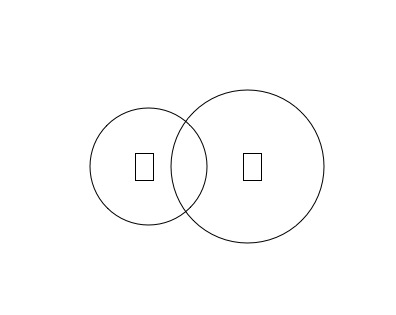
\includegraphics[width=2.5in]{./img/sensorDistance.jpg}
\caption{SensorDistance.}
\label{fig_sim}
\end{figure}

In opportunistic networks [T], node-to-node communication occurs by exploiting any tidbit of connectivity that becomes available. Nodes in an opportunistic network rely on pairwise encounters and a store-and-forward paradigm to send information to each other over multiple hops even in the absence of an end-to-end path. Opportunistic communication is possible as long as there are foris no longer viewed as a disruptive phenomenon that thwarts the laborious routing process, but as a benefit that streamlines communication by offering new data exchange opportunities between nodes. Mobility enables nodes to come in contact with other nodes and makes it more likely for them to encounter useful forwarders that can get their messages closer to its intended destination.
Thewarding opportunities. By breaking away from any end-to-end path requirement, opportunistic networks lend themselves to the pervasive vision by making connectivity available anywhere and anytime, though not all the time. Any user can exchange data with any other user from any location at any time, as long as she is not a hermit and is in no hurry. Opportunistic networks allow information to flow to its destination through the combined use of network connectivity and node mobility. Mobility is no longer viewed as a disruptive phenomenon that thwarts the laborious routing process, but as a benefit that streamlines communication by offering new data exchange opportunities between nodes. Mobility enables nodes to come in contact with other nodes and makes it more likely for them to encounter useful forwarders that can get their messages closer to its intended destination [1].
Fig. 1 illustrates the working procedure of the Crowd Foraging framework. In an opportunistic network scenario, amobile task requester R launches a mobile crowdsourcing task. She moves around in the network and opportunistically encounters a mobile human worker W1.After probing the work ability of the worker W1 via D2D link, if the task requester R decides to recruit the worker in terms of a specific recruitment policy, she will forward the detailed contents of the task (e.g., images, videos and text descriptions) to the recruited worker via D2D link. Once the worker finishes the task, he will send the results to the task requester via either cellular link directly or D2D link when they encounter with each other again before a given deadline. Finally, the task requester receiving the results will grant the task reward to the worker. We should emphasize that, our framework only considers one-hop mechanism for both worker recruitment and result collection, since realistic dataset analyses reveal that users’ one-hop neighbors are sufficient [7] and can cover most range of the whole network in a reasonable time period [10], and contacting a user would incur long delay if the maximum D2D communication hops are larger than two [15]. Compared with multi-hop mechanisms in existing researches [1], [3], [4], [6], [11], [12], this one-hop feature can lower the network overhead (e.g., no need to transfer a large volume of task contents hop by hop) and ensure framework performance with only local information, which ismore practical in real life[3].

In this section, we introduce MSSC that is a virtual community formed by multiple mobile users. Within it, users can share services on their own mobile devices through mobile networks. It has three main characteristics as follows.

1) Locality: An MSSC is not established on the Internet. It corresponds to a specific region such as a univer- sity campus, a company building, and a restaurant. Only mobile users who enter the same region can share services with each other.

2) Dynamicity: MSSC participants are not stationary. They can enter or leave the community at any time.

3) Mobility: Services provided by mobile users are not fixed at the same location. Service requesters are also mobile when invoking a mobile service.

In order to provide more details for MSSC, this section gives its basic architecture, operations, and applications.
\subsection{Overview}
[2]
\subsection{Basic Operations}
[2]
\subsection{Application Scenario}
[2]

\section{SERVICE COMPOSITION OVER MON APPROACH}
\subsection{Node Availiable for Opportunistic network}
In wireless mobile networks such as ad hoc or mesh networks, the availability of a node to its neighbour nodes is highly related to the node’s mobility—here it is assumed that battery power is not a concern and as such a node will not out of reach because of battery exhaustion. If node i moves outside the transmission range of its neighbouring node j, then node i is unreachable by node j and as a result the services on node i become unavailable to node j either. Node availability, to some extent, also expresses network availability because if the connection between any two neighbouring nodes in a route from a service provider to a service requester becomes unavailable, then the whole route also becomes unavailable. Here node mobility is utilized to calculate the node availability [4].

Consider, as illustrated in Fig. 2, two mobile hosts MHi
and MHj of the same transmission range R. Each node moves randomly and it is assumed that the moving field is a circle with a radius of r. d represents the distance between MHi and MHj. These three parameters are to be used for calculating the node availability. The transmis- sion range of a node R is known (e.g., pre-defined or changing according to certain algorithm). Suppose the location (i.e., coordinates) of each mobile host is known (e.g., via GPS—global positioning system), then distance d can be calculated using the Euclidean distance formula, i.e.,$\sqrt{{(x_i-x_j)^2}+{y_i-y_j}^2}$ where $(x_i, x_j)$ and $(y_i, y_j)$ are are the coordinates of MHi and MHj respectively. Finally let us discuss how to calculate r.

The moving radius of a mobile host (r) is its speed (s) multiplied by the average service time (t). Here t can be statistically calculated as the average value of last n servings of this component service, namely, $t = \Sigma_{i=1}^{n}t_i/n$. The speed of a mobile host s can be calculated based on its moving distance during a period from t1 to t2 [18], namely: $s = \sqrt{{(x_i-x_j)^2}+{y_i-y_j}^2}/(t_2-t_1)$. Then $r = s \times t$.

Knowing the values of these three parameters R, r,
and d, the probability of MHi staying inside the transmission range of MHj (denoted as $P_i^{IN}$ ) can be calculated by

\begin{equation}
P_i^{IN} = \frac{A_i^{IN}}{A_i^T}
\end{equation}

Namely, $P^{IN}_i$ equals to the area of the MHi’smoving field inside the transmission range of MHj (denoted as $A^{IN}_i$) divided by the overall area of the MHi’s moving field($A^T_i$).

As shown in Fig. 2, we have

\begin{equation}
\alpha = arcons(\frac{r^2+d^2-R^2}{2r\times d})
\end{equation}

\begin{equation}
\beta = arcons(\frac{R^2+d^2-r^2}{2r\times d})
\end{equation}

Then, 
\begin{eqnarray}
A^{IN}_i = [(\frac{2\beta}{2\pi}\pi R^2)-(\frac{R sin\beta cos\beta}{2}2)]\\\nonumber
+ [(\frac{2\alpha}{2\pi}\pi r^2)-(\frac{r sin\alpha cos\alpha}{2}2)]\\\nonumber
= \beta R^2 + \alpha r^2 - (R^2 sin\beta cos\beta + r^2 sin\alpha cos\alpha)
\end{eqnarray}

There is also
\begin{equation}
A_i^T = \pi r^2 = \pi \times (s \times t)^2
\end{equation}

Therefore, we obtain
\begin{equation}
P_i^{IN} = \frac{A_i^{IN}}{\pi s^2 t^2}
\end{equation}

The probability of MHi staying inside the transmission range of $MH_j (P^{IN}_i)$ can be calculated. Suppose service $s$ running on MHi is a candidate service for a task running on MHj, and the node availability with regard to service s is denoted as $q_{av}^n(s)$, then finally there is
\begin{eqnarray}
q_{av}^n(s) = P^{IN}_i = \frac{A_i^{IN}}{\pi s^2 t^2}\\\nonumber
= \frac{\beta R^2 + \alpha r^2 - (R^2 sin\beta cos\beta + r^2 sin\alpha cos\alpha)}{\pi s^2 t^2}
\end{eqnarray}

\subsection{Problem Description}
In order to describe the problem addressed in this paper, we first provide formal definitions of a few key concepts in MSSC and then present the problem description.

Definition 3 (Mobile User): Amobile user isa four-tuple
u = (uid, umt, S, l) where uid is the identification;
umt is the moving trajectory;
S   is a set of mobile services that u can provide where S can be a null set if u does not want to share its own services;
l   is the sensing distance of u’s mobile device.


Definition 4 (Mobile Service): A mobile service is a triple
s = (sid, e) where sid is the identification;
e is the response time.
Service providers publish the information of their services including function and nonfunction properties. So the average response time of a service is already known when a requester selects it. For data-intensive services, the response time is afunction of the input data. To simplifythe explanation, we assume that the response time of a mobile service is a constant.

Definition 5 (Composition Request): Acomposition request
is a two-tuple cr = (T, R)where T ={t1, t2,..., tn}
is a set of tasks;
R ={r(ti, tj)|ti, tj ∈ T} is a set of relations between tasks in T.
Each task ti can be implemented by a set of candidate ser-
vices, and r(ti, tj) = 1 represents that the inputs of tj depend on the outputs of ti. R is used to describe the structure of the
composition.

Definition 6 (Mobile Service Composition): A mobile ser-
vice composition is a triple msc = (h, S, L), where h
is the composition request to which msc corre- sponds;
S is the set of services in msc;
$L = \coprod_{s \in S} l_s$ is the total response time of msc.

Definition 7 (MSSC Service Composition): Given a mobile service sharing community mssc, and a service composition request h by a mobile user u,select concrete servicespro- vided by other mobile users in MSSC to achieve an optimal service composition msc with the shortest response time L. Meanwhile, msc should guarantee to run successfully when the service requester and the service providers are moving.

Theorem 1: The service composition problem in MSSC (Definition 6) is NP-hard.
Proof: The standard integer program to find the smallest value of a given objective function $F(\Theta)$ with a feasible parameter vector $\Theta = (\theta_1,..., \theta_n)$ can be given as follows [21]:

\begin{eqnarray}
inf F(\Theta)\\\nonumber
subject \ to \  \theta_i \in \{1,2,3,...,N\}.
\end{eqnarray}
This means that the feasible set of parameter vectors is con-
strained by θi ∈ {1, 2,...,N} with integer values. The optimal solution ?∗ satisfies the following conditions.
1) ?∗ belongs to the feasible set.
2) ∀?,F(?∗) ≤ F(?). For the problem of selecting optimal services with shortest response time while considering mobility, the vector ? = (θ1,..., θn) can describe a possible solution as a service composition with n tasks. An element θi in ? corresponds to aselected service from thecandidates for the ith task [2].

The target of the mobile service composition problem in
MSSC is to find ? to obtain the smallest F(?).Thus, the problem is equivalent to the integer program described in (2). An integer programming problem is known to be NP-hard. Then the service composition problem in MSSC is NP-hard. For such a problem, integer programming can be utilized to
obtain the optimal solution. However, they might cost much time when the problem size increases. In mobile environment, the requirement on runtime is essential since the environment parameters for computation may vary much within a short time. Therefore, although integer programming can obtain the optimal result, it is not suitable to the problem due to its poor scalability. So one possible way to obtain a satisfactory solu- tion in an accepted execution time is to design a heuristic search method and find the near optimal solution. For exam- ple, metaheuristic algorithms such as GAs and PSO, can be utilized to solve this problem. Among them, we find that KH algorithm can reduce the search space and return high approx- imate optima. Thus, we propose a solution method based on it to find an approximate optimal solution in polynomial time[2].

\subsection{Composition Algorithm}
In this section, we solve the proposed problem by using a heavily tailored GA. The genetic encoding, fitness function, and genetic operators are described in Sections V-B1–V-B3. The whole algorithm is shown in Section V-B4 [6].

1) Genetic Encoding: In GA, a genome is a genetic rep- resentation of the solution, and for our problem, a concrete composite service instance is encoded as a genome. The genome is represented by an array whose length is equal to the number of involved services. The ith entry in the array (i.e., ith gene in the genome) refers to the selection result of the ith service. That is to say, given that the value of the ith entry is j,itindicates that si,j, i.e., the jth candidate in gcnd(si), is selected to execute si [6]. 

2) Fitness Function: The fitness function is defined over the genome and measures the fitness of the represented solution. As clarified in Section IV-D, the fitness of a composite service instance csi depends on its QoS utility and on whether the end-to-end QoS constraints are satisfied

The penalty technique is used to drive the evolution toward constraint satisfaction [48]. In this paper, the penalty function is defined in (4)and (5), and it measures the negative total nor- malized distance from q(csi) to the QoS constraints qc when the constraint is violated. Then, in (6), the fitness function is defined as the weighted sum of the QoS utility U(csi) and the penalty function P(csi), where the penalty weight (wpen×gen) increases with the generation number gen. In so doing, in the early generations, genomes violating the constraints but with high utility values can still be considered, and in the late generations, genomes violating the constraints are severely punished

\begin{equation}
P(csi) = - \sum_{q_t \in Q} \frac{\Delta q_t}{q_{t,max} - q_{t,min}}
\end{equation}

\begin{equation}
\Delta q_t = 
\left\{ 
\begin{array}{cc}
qc_t - q_t(csi)  if ... \\
qc_(csi) - qc_t  if ... \\
0 \  else ... \\
\end{array} 
\right. 
\end{equation}


\begin{equation}
F(csi) = U(csi) + w_{pen} + gen + P(csi)
\end{equation}

3) Genetic Operators: To guarantee that each genome in the population is always valid, we extend each genetic operator with special adaptation. 

a) Initialization operator: An empty array with a length equal to the number of services is initialized and random assignment is performed from the first gene to the last. An instance c from the generalized candidates gcnd(s1) of s1 is randomly selected and bound to the first gene. If gra(c) ≥ 2, the following gra(c)-1 genes are assigned a $\#$. After that, the ith gene [i = 1 + gra(c)]is selectedto beassigned, and this process loops until the last gene is assigned [6].

b) Crossover operator: For a genome of length n,there are n − 1splitting pointsin total. However, choosing some of them as splitting points will render the resulting genome invalid after crossover, and thus in a genome, the genes belong- ing to the same coarse-grained service instance should not be split. Let sp1 be the set of feasible splitting points in parent1,and sp2 be that for parent2.The splitting points that the crossover operator can use are limited to the intersection of sp1 and sp2.For instance, in Fig. 7,sp1 is {1, 3, 4, 5, 6} and sp2 is {1, 2, 3, 7}, and thus, the splitting points that the crossover operator can use is {1, 3}. Note that this intersec- tion may be empty, and in this case, the two parents will be directly copied to the offspring [6].


c) Mutation operator: Mutation is used to maintain genetic diversity from one generation of a population to the next. Traditionally, each gene in the genome is selected and mutated with the same probability and in this case, coarse- grained service instances would more likely be replaced. Instead, a service instance is randomly selected with the same probability from all the service instances contained in the rep- resented solution and the corresponding genes of the selected instance are marked to be mutated. Let i be the position of the first marked gene, and c be a new candidate randomly selected from gcnd(si)to replace theoriginal one. If gra(c)is not greater than the number of marked genes, c is assigned to the ith gene and the gene is unmarked. In addition, the following gra(c) − 1genes areassigned a$\#$and are unmarked. Otherwise, it indicates that the selected instance conflicts with existing service instances in the genome.Whether c is adopted or not can lead to quite different results [6].

\section{SIMULATION AND EVALUATION}
\subsection{Simulation Setting}
\subsection{Scalability Evaluation}
\subsection{Effectiveness Evaluation}
\section{CONLUSION}







\ifCLASSOPTIONcaptionsoff
  \newpage
\fi



\begin{thebibliography}{1}

\bibitem{IEEEhowto:Giordano}
Giordano, S., and Puccinelli, D. (2011). The Human Element as the Key Enabler of Pervasiveness, 150–156.

\bibitem{}
Deng, S., Huang, L., Taheri, J., Yin, J., Zhou, M., and Zomaya, A. Y. (2017). Mobility-aware service composition in mobile communities. IEEE Transactions on Systems, Man, and Cybernetics: Systems, 47(3), 555–568.

\bibitem{}
Pu, L., Chen, X., Xu, J., and Fu, X. (2017). Crowd Foraging : A QoS-Oriented Self-Organized Mobile Crowdsourcing Framework Over Opportunistic Networks, 35(4), 848–862.

\bibitem{}
Yang, K., Galis, A., and Chen, H.-H. (2010). Qos-aware service selection algorithms for pervasive service composition in mobile wireless environments. Mobile Networks and Applications, 15(4), 488–501.

\bibitem{}
Zhang, C., Zhang, L., and Zhang, G. (2016). QoS-Aware Mobile Service Selection Algorithm, 2016.

\bibitem{}
Wu, Q., Ishikawa, F., Zhu, Q., and Shin, D.-H. (2016). QoS-Aware Multigranularity Service Composition: Modeling and Optimization. IEEE Transactions on Systems, Man, and Cybernetics: Systems, 46(11), 1565–1577.

\end{thebibliography}

\end{document}


